This chapter presents a review of the main theoretical aspects involved
in the formulation, estimation, and implementation of a generalized
linear mixed model (GLMM). We start in \autoref{cap:joint} with the
model formulation framework, concluding with the so-called joint or full
likelihood function. \autoref{cap:laplace} address the marginalization
of that joint likelihood, performed here in terms of a Laplace
approximation technique. \autoref{cap:opt} discusses available
alternatives for the marginal likelihood parameters optimization.
\autoref{cap:ad} present the automatic differentiation (AD) procedure,
the most efficent routine for the computation of derivatives, and a key
point for us. Last but not least, in \autoref{cap:tmb} we present the
computational tool used for the discussed methodology, a very
exciting \texttt{R} \cite{R21} package called TMB: Template Model
Builder, developed by~\citeonline{TMB}.

\section{FORMULATION: OBTAINING A JOINT LIKELIHOOD FUNCTION}
\label{cap:joint}

We model an \(n\)-vector of exponential family random variables
\(\bm{Y}\), in terms of its conditional expected value \(\bm{\mu} \equiv
\mathbb{E}(\bm{Y} \mid \bm{X,u})\), via a linear combination called of
linear predictor and generally expressed by
\begin{equation}
 g(\bm{\mu}) = \bm{X\beta} + \bm{Zu}, \quad
 \bm{u} \sim \text{Multivariate Normal}(\bm{0,\Sigma}).
 \label{eq:gmu}
\end{equation}
In other words, a GLMM \cite{GLMM} is a generalized linear model (GLM)
in which the linear predictor depends on some Gaussian latent effects,
\(\bm{u}\), times a latent effects design-matrix \(\bm{Z}\). Since we do
not observe the latent component, an exemplification of the idea
embedded in matrix \(\bm{Z}\) is welcome. Suppose e.g., three
individuals (or clusters) and that each one has two measures. This
configures a repeated measures context, the most common latent structure
in family studies. Also, it is reasonable to admit that each individual
has its particular latent effect value. Consequently, we have
\[
 \bm{Zu} = \begin{bmatrix}
            1 & 0 & 0\\1 & 0 & 0\\
            0 & 1 & 0\\0 & 1 & 0\\
            0 & 0 & 1\\0 & 0 & 1\\
           \end{bmatrix} \begin{bmatrix}
                          u_{1}\\u_{2}\\u_{3}\\
                         \end{bmatrix} = \begin{bmatrix}
                                          u_{1}\\u_{1}\\
                                          u_{2}\\u_{2}\\
                                          u_{3}\\u_{3}\\
                                         \end{bmatrix},
\]
where \(\bm{u}^{\top} = [u_{1}~u_{2}~u_{3}]\) and \(\bm{Z}\) has the
role of projecting the values of \(\bm{u}\) to match the number of
measures.

In a mixed model the mean structure is approached as a combination of
probability distributions. It is a combination since we have to assume
probabilistic structures for the observed and non-observed/latent data.
To each observed variable \(y_{ij}\) we have a probability distribution
of the exponential family, denoted by \(f(y_{ij} \mid \bm{u}_{i},
\bm{\theta})\). To the latent effect we have, generally, a
(multivariate) Gaussian distribution, denoted by \(f(\bm{u}_{i} \mid
\bm{\Sigma})\). To each individual or unity under study \(i\), and to
each measure \(j\), we have the product of these probability densities,
a likelihood contribution.

Our goal is to estimate the parameter vector \(\bm{\theta} =
[\bm{\beta~\Sigma}]^{\top}\) of a mean structure, as in
\autoref{eq:gmu}. Besides the role of emphasizing the fact that
\(\bm{\mu}\) is a function of \(\bm{\theta}\), and that we want to
estimate \(\bm{\theta}\), the likelihood function ties the probability
densities i.e., the likelihood is the product of the product of
probability densities, to each subject \(i\). Since \(Y_{i}\) are
mutually independent, the likelihood for \(\bm{\theta}\) can be written
as
\begin{equation}
 L(\bm{\theta} \mid \bm{y,u}) =
 \prod_{i=1}^{I}~\prod_{j=1}^{n_{i}}~
 f(y_{ij} \mid \bm{u}_{i}, \bm{\beta,\Sigma})~
 f(\bm{u}_{i} \mid \bm{\Sigma}).
 \label{eq:joint}
\end{equation}
From standard probability theory is easy to see that in the right-hand
side (r.h.s.) we have a joint density, consequently, \autoref{eq:joint}
represents what is called a full or a joint likelihood function. What
makes problematic working with this joint likelihood is that we do not
have all the necessary information to just maximize it and get the
desired parameter estimates. The latent effect \(\bm{u}\) is
\textit{latent} i.e., we do not observe it. To handle this we have
basically two available paths.

\section{MARGINALIZATION: LAPLACE APPROXIMATION AND ALTERNATIVES}
\label{cap:laplace}

To deal with a joint likelihood function as in \autoref{eq:joint} we
have a choice to make. Be or not to be Bayesian. Each choice has its own
difficulties, advantages, and characteristics.

The Bayesian path assumes that all \(\bm{\theta}\) components are random
variables. With all parameters being treated as random variables, and
since we do not observe them, what the Bayesian framework does is try to
compute the mode of each ``parameter'' marginal distribution, generally,
via a sampling algorithm called MCMC: Markov chain Monte Carlo
\cite{MCMC, Diaconis}.

The advantage of being Bayesian is that we can reach an MCMC algorithm
to basically any statistical model, the disadvantage is that this
approach is very time consuming and we have to propose prior
distributions to each ``parameter''. These prior proposals are not
always easy to make, and the resulting marginal distributions can be
very depending of it. A Bayesian approach can be applied in basically
any context, without guarantees that will work - obtain convergence to
all parameters is not a straightforward task. However, in complex
scenarios they can be the only available method to ``maximize'' the
likelihood function. This is not the case here.

We have a joint density where one of the random variables is not
observed, but we are not interested in it, only in the variance
parameters inherent in it. Again, from standard probability theory, if
we have a joint density we can just integrate out the undesired variable
resulting in
\begin{equation}
 \begin{aligned}
  L(\bm{\theta} \mid \bm{y}) &=
  \prod_{i=1}^{I}~\int_{\mathcal{R}^{\bm{u}_{i}}}
  \left[~\prod_{j=1}^{n_{i}}~
         f(y_{ij} \mid \bm{u}_{i}, \bm{\beta,\Sigma})~
         f(\bm{u}_{i} \mid \bm{\Sigma})
  \right]\text{d} \bm{u}_{i}\\
  &= \prod_{i=1}^{I}~\int_{\mathcal{R}^{\bm{u}_{i}}}~
  f(\bm{y}_{i}, \bm{u}_{i} \mid \bm{\theta})~\text{d} \bm{u}_{i},
  \label{eq:generalmarginal}
 \end{aligned}
\end{equation}
a marginal density that keeps the parameters \(\bm{\Sigma}\) of the
integrated variable.

When the response distribution of a mixed model is Gaussian, is
analytically tractable to integrate \(\bm{u}\) out of the joint density.
Consequently, it is possible to evaluate the marginal likelihood
exactly. This is the case of the linear mixed models (LMMs) and one of
the main differences to the GLMMs. When the response distribution is not
Gaussian, generally, it is not anymore analytically tractable to
integrate out the latent effect. So what do we do? Well, we have
basically two options again.

We can avoid the integrals in \autoref{eq:generalmarginal}, replacing it
by integrals that are tractable. This can be performed via an algorithm
called Expectation-Maximization (EM), proposed by
\citeonline{EM77}. This approach is considered a little bit naive and
generally is not recommended if you have a better option. The other
option consists of performing a numerical integration i.e.,
approximating the integral. The most common way of doing that in the
statistical modeling literature is via an importance sampling version of
the Gaussian quadrature rule, denoted adaptive Gaussian quadrature (AGQ)
\cite{quadrature}. In general, adaptive Gaussian quadratures are not so
simple to use (computationally expensive; we have to choose how many
integration points will be used; and we also have to choose an
importance distribution to approximate the integrand).

To us, the better option consists in take advantage of the exponential
family structure together with the fact that we are dealing with
Gaussian latent effects. These ideas converge to an adaptive Gaussian
quadrature with one integration point, also called as \textit{Laplace
approximation}
\cite{molenberghs&verbeke, LA4H, tierney, corestats}.

With an integral that is analytically intractable, we may approximate it
to obtain a tractable closed-form expression allowing the numerical
maximization of the resulting marginal likelihood function
\cite{patrao}. The Laplace approximation has been designed to
approximate integrals in the form
\begin{equation}
 \int_{\mathcal{R}^{\bm{u}_{i}}}
 \exp\{Q(\bm{u}_{i})\} \text{d} \bm{u}_{i}\approx
 (2\pi)^{n_{\bm{u}}/2}~
 |{Q}''(\bm{\hat{u}}_{i})|^{-1/2}~\exp\{Q(\bm{\hat{u}}_{i})\},
 \label{eq:laplace}
\end{equation}
where \(Q(\bm{u}_{i})\) is a known, unimodal bounded function, and
\(\bm{\hat{u}}_{i}\) is the value for which \(Q(\bm{u}_{i})\) is
maximized. As \citeonline{corestats} shows, a Laplace approximation
consists of a second order Taylor expansion of \(\log f(\bm{y}_{i},
\bm{u}_{i} \mid \bm{\theta})\), about \(\bm{\hat{u}}_{i}\), that gives
\[
 \log f(\bm{y}_{i}, \bm{u}_{i} \mid \bm{\theta})\approx
 \log f(\bm{y}_{i}, \bm{\hat{u}}_{i} \mid \bm{\theta}) -
 \frac{1}{2} (\bm{u}_{i} - \bm{\hat{u}}_{i})^{\top}\bm{H}~
             (\bm{u}_{i} - \bm{\hat{u}}_{i}),
\]
where \(\bm{H} = - \nabla_{u}^{2} \log f(\bm{y}_{i}, \bm{\hat{u}}_{i}
\mid \bm{\theta})\). Hence, we can approximate the joint by
\begin{equation}
 f(\bm{y}_{i}, \bm{u}_{i} \mid \bm{\theta})\approx
 f(\bm{y}_{i}, \bm{\hat{u}}_{i} \mid \bm{\theta})~\exp
 \left\{-\frac{1}{2} (\bm{u}_{i} - \bm{\hat{u}}_{i})^{\top}\bm{H}~
                     (\bm{u}_{i} - \bm{\hat{u}}_{i})
 \right\}.
 \label{eq:taylor}
\end{equation}
From here we start to take advantage of the points mentioned above.

First, the fact that we are dealing with Gaussian distributed latent
effects. In \autoref{eq:taylor} we have the core of a Gaussian density,
that complete is
\[
 \int_{\mathcal{R}^{\bm{u}_{i}}}
 \frac{1}{(2\pi)^{n_{\bm{u}}/2}~|\bm{H}^{-1}|^{1/2}}~\exp
 \left\{-\frac{1}{2} (\bm{u}_{i} - \bm{\hat{u}}_{i})^{\top}\bm{H}~
                     (\bm{u}_{i} - \bm{\hat{u}}_{i})
 \right\} \text{d} \bm{u}_{i} = 1
\]
i.e., integrates to 1. Integrating \autoref{eq:taylor} follows that
\begin{align*}
 \int_{\mathcal{R}^{\bm{u}_{i}}}
 f(\bm{y}_{i}, \bm{u}_{i} \mid \bm{\theta})~\text{d} \bm{u}_{i}
 &\approx f(\bm{y}_{i}, \bm{\hat{u}}_{i} \mid \bm{\theta})
  \int_{\mathcal{R}^{\bm{u}_{i}}}
  \exp \left\{-\frac{1}{2}
               (\bm{u}_{i} - \bm{\hat{u}}_{i})^{\top}\bm{H}~
               (\bm{u}_{i} - \bm{\hat{u}}_{i})
       \right\} \text{d} \bm{u}_{i}\\
 &= (2\pi)^{n_{\bm{u}}/2}~|\bm{H}|^{-1/2}~
    f(\bm{y}_{i}, \bm{\hat{u}}_{i} \mid \bm{\theta})
\end{align*}
i.e., we get \autoref{eq:laplace}, a first order Laplace approximation
to the integral. Careful accounting of the approximation error shows it
to generally be \(\mathcal{O}(n^{-1})\), where \(n\) is the sample size,
and assuming a fixed length for \(\bm{u}_{i}\) \cite{corestats}.

The second advantage of a Laplace approximation approach in a GLMM is
the exponential family structure. In a usual GLMM the response follows a
one-parameter exponential family distribution that can be written as
\[
 f(\bm{y}_{i} \mid \bm{u}_{i}, \bm{\theta}) =
 \exp \left\{
  \bm{y}_{i}^{\top} (\bm{x}_{i}\bm{\beta} + \bm{z}_{i}\bm{u}_{i}) -
  \bm{1}_{i}^{\top}b(\bm{x}_{i}\bm{\beta} + \bm{z}_{i}\bm{u}_{i}) +
  \bm{1}_{i}^{\top} c(\bm{y}_{i})
      \right\},
\]
where \(b(\cdot)\) and \(c(\cdot)\) are known functions.

This general and easy to compute expression, together with a
(multivariate) Gaussian distribution, highlights the convenience of the
Laplace method. The \(Q(\bm{u}_{i})\) function to be maximized can be
expressed as
\begin{equation}
 \begin{aligned}
  Q(\bm{u}_{i}) &=
  \bm{y}_{i}^{\top} (\bm{x}_{i}\bm{\beta} + \bm{z}_{i}\bm{u}_{i}) -
  \bm{1}_{i}^{\top}b(\bm{x}_{i}\bm{\beta} + \bm{z}_{i}\bm{u}_{i}) +
  \bm{1}_{i}^{\top} c(\bm{y}_{i})\\
  &- \frac{n_{\bm{u}}}{2} \log (2\pi) -
     \frac{1}{2} \log |\bm{\Sigma}| -
     \frac{1}{2} \bm{u}_{i}^{\top}\bm{\Sigma}^{-1}~\bm{u}_{i}.
 \end{aligned}
\end{equation}
The approximation in~\autoref{eq:laplace} requires the maximum
\(\bm{\hat{u}}_{i}\) of the function \(Q(\bm{u}_{i})\). As we assume a
Gaussian distribution with a known mean for the latent effects, we have
the perfect initial guess for a Hessian-based maximization method, as
the Newton-Raphson (NR) algorithm.

The NR method consists of an iterative scheme as follows:
\[
 \bm{u}_{i}^{(k+1)} =
 \bm{u}_{i}^{(k)} - {Q}''(\bm{u}_{i}^{(k)})^{-1}~{Q}'(\bm{u}_{i}^{(k)}),
 \quad k = 0,~1,~\dots
\]
until convergence, which gives \(\bm{\hat{u}}_{i}\). At this stage, all
parameters \(\bm{\theta}\) are considered known. \citeonline{patrao}
presents the generic expressions for the derivatives required by the NR
method, given by the following:
\begin{equation}
 \begin{aligned}
  {Q}'(\bm{u}_{i}^{(k)}) &=
  \{\bm{y}_{i} - {b}'(\bm{x}_{i}\bm{\beta} + \bm{z}_{i}\bm{u}_{i}^{(k)})
  \}^{\top} - {\bm{u}_{i}^{(k)}}^{\top} \bm{\Sigma}^{-1},\\
  {Q}''(\bm{u}_{i}^{(k)}) &=
  - \text{diag}\{{b}''(\bm{x}_{i}\bm{\beta}
  + \bm{z}_{i}\bm{u}_{i}^{(k)})\} - \bm{\Sigma}^{-1}.
 \end{aligned}
 \nonumber
\end{equation}
We have the initial guesses at \(k = 0\).

Finally, the marginal log-likelihood function returned by the Laplace
approximation, to each individual or unit under study \(i\), is as
follows:
\begin{equation}
 \begin{aligned}
  l(\bm{\theta} \mid \bm{y}_{i}) =
  \log L(\bm{\theta} \mid \bm{y}_{i}) &= \frac{n}{2} \log (2\pi) -
  \frac{1}{2} \log
  \left| \text{diag}\{{b}''(\bm{x}_{i}\bm{\beta} +
                      \bm{z}_{i}\bm{\hat{u}}_{i})
                    \} + \bm{\Sigma}^{-1}
  \right|\\
  &+ \bm{y}_{i}^{\top}
     (\bm{x}_{i}\bm{\beta} + \bm{z}_{i}\bm{\hat{u}}_{i}) -
     \bm{1}_{i}^{\top}
     b(\bm{x}_{i}\bm{\beta} + \bm{z}_{i}\bm{\hat{u}}_{i}) +
     \bm{1}_{i}^{\top} c(\bm{y}_{i})\\
  &- \frac{n_{\bm{u}}}{2} \log (2\pi) -
     \frac{1}{2} \log |\bm{\Sigma}| - \frac{1}{2}
     \bm{\hat{u}}_{i}^{\top}\bm{\Sigma}^{-1}~\bm{\hat{u}}_{i},
 \end{aligned}
 \nonumber
\end{equation}
that can now be numerically maximized over the model parameters
\(\bm{\theta} = [\bm{\beta~\Sigma}]^{\top}\).

\section{OPTIMIZATION: MARGINAL LIKELIHOOD FUNCTION}
\label{cap:opt}

At this point it is already clear that we have two optimizations to be
performed, an ``inside'' and an ``outside'' optimization. The inside one
is made into the Laplace approximation layer via a Newton-Raphson
algorithm, a Newton's method. The outside optimization is made with the
Laplace approximation outputs i.e., the maximization of
\autoref{eq:generalmarginal}'s marginal log-likelihood over its
parameters \(\bm{\theta}\). This task is usually performed via a
quasi-Newton method, we focus on two of the most traditional ones: the
Broyden-Fletcher-Goldfarb-Shanno (BFGS) algorithm and the PORT routines.

The inside optimization is the numerical maximization of the joint
log-likelihood with respect to (w.r.t.) its latent effects. This is kind
of a simple task since all model parameters are considered as fixed, and
we ``know'' that the latent effects are distributed with zero mean i.e.,
we have the perfect initial guess. In this context, the use of a
Newton's method is straightforward. When we talk about the outside
optimization it is a completely different scenario, it is not
straightforward to find a good initial guess or reach convergence. Thus,
more robust methods are a good choice.

In optimization, Newton methods are algorithms for finding local maxima
and minima of functions i.e., the search for the zeroes of the gradient
of that function. Newton methods are characterized by the use of a
symmetric matrix of function's second derivatives, the Hessian matrix.
Quasi-Newton methods are based on Newton's method and are seen as an
alternative to it. They can be used if the Hessian is unavailable or if
is too expensive to compute it at every iteration.

As shown in \citeonline{nocedal&wright}, major advantages of
quasi-Newton methods over Newton's method are that the Hessian matrix
does not need to be computed, it is approximated; and it also does not
need to be inverted. Newton's method requires the Hessian to be
inverted, typically by solving a system of linear equations - often
quite costly. In contrast, quasi-Newton methods usually generate an
estimate of it directly. As in Newton's method, they use a second-order
approximation to find the minimum of a function \(f(\bm{x})\). The
Taylor series of \(f(\bm{x})\) around an iterate is
\[
 f(\bm{x}_{k} + \Delta\bm{x})\approx
 f(\bm{x}_{k}) + \nabla f(\bm{x}_{k})^{\top}\Delta\bm{x} +
 \frac{1}{2} \Delta\bm{x}^{\top}\bm{B}~\Delta\bm{x},
\]
where \(\nabla f(\cdot)\) is the gradient, and \(\bm{B}\) an
approximation to the Hessian matrix. The gradient of this approximation
w.r.t. \(\Delta\bm{x}\) is
\[
 \nabla f(\bm{x}_{k} + \Delta\bm{x}) \approx
 \nabla f(\bm{x}_{k}) + \bm{B}~\Delta\bm{x},
\]
setting this gradient to zero provides the Newton step:
\[
 \Delta\bm{x} = - \bm{B}^{-1}\nabla f(\bm{x}_{k}).
\]
The Hessian approximation \(\bm{B}\) is chosen to satisfy
\[
 \nabla f(\bm{x}_{k} + \Delta\bm{x}) =
 \nabla f(\bm{x}_{k}) + \bm{B}~\Delta\bm{x},
\]
which is called the \textit{secant} equation i.e., the Taylor series of
the gradient itself. Solving for \(\bm{B}\) and applying the Newton's
step with the updated value is equivalent to the \textit{secant} method.
Quasi-Newton methods are a generalization of the secant method to find
the root of the first derivative for multidimensional problems. The
various quasi-Newton methods differ in their choice of the solution to
the secant equation.

In a general quasi-Newton method, the unknown \(\bm{x}_{k}\) is
updated applying the Newton's step calculated using the current
approximate Hessian matrix \(\bm{B}_{k}\) in the following fashion:
\begin{itemize}
 \item \(\Delta \bm{x}_{k} = -\alpha_{k}\bm{B}_{k}^{-1}\nabla
       f(\bm{x}_{k})\), with \(\alpha\) chosen to satisfy some
       sufficient decrease and curvature conditions collectively known
       as the \textit{Wolfe conditions} \cite[p.~34]{nocedal&wright};

 \item \(\bm{x}_{k+1} = \bm{x}_{k} + \Delta\bm{x}_{k}\);

 \item The gradient computed at the new point \(\nabla
       f(\bm{x}_{k+1})\), and \(\bm{y}_{k} = \nabla f(\bm{x}_{k+1}) -
       \nabla f(\bm{x}_{k})\) is used to update the approximate Hessian
       \(\bm{B}_{k+1}\), or directly its inverse
       \(\bm{H}_{k+1} = \bm{B}_{k+1}^{-1}\).
\end{itemize}

The most popular quasi-Newton method is the BFGS algorithm, named after
its inventors, Broyden, Fletcher, Goldfarb, and Shanno. It has the
following update formula
\begin{align*}
 \bm{B}_{k+1} &= \bm{B}_{k} +
                \frac{\bm{y}_{k}\bm{y}_{k}^{\top}}{
                      \bm{y}_{k}^{\top}\Delta\bm{x}_{k}} -
                \frac{\bm{B}_{k}\Delta\bm{x}_{k}
                     (\bm{B}_{k}\Delta\bm{x}_{k})^{\top}}{
                      \Delta\bm{x}_{k}^{\top}\bm{B}_{k}
                      \Delta\bm{x}_{k}},\\
 \bm{H}_{k+1} = \bm{B}_{k+1}^{-1}
            &= \left(\bm{I} -
                     \frac{\Delta\bm{x}_{k}\bm{y}_{k}^{\top}}{
                           \bm{y}_{k}^{\top}\Delta\bm{x}_{k}}
                \right) \bm{H}_{k}
                \left(\bm{I} -
                      \frac{\bm{y}_{k}\Delta\bm{x}_{k}^{\top}}{
                            \bm{y}_{k}^{\top}\Delta\bm{x}_{k}}
                \right) + \frac{\Delta\bm{x}_{k}
                                \Delta\bm{x}_{k}^{\top}}{
                                \bm{y}_{k}^{\top}\Delta\bm{x}_{k}}.
\end{align*}
Another quasi-Newton method popular in the statistical modeling
literature, is the one based on the PORT routines
\url{http://www.netlib.org/port/}. It is a Fortran mathematical
subroutine library designed to be \textit{portable} over different types
of computers, developed by David Gay in the Bell Labs \cite{PORTreport}.
It is a quasi-Newton adaptive nonlinear least-squares algorithm
\cite{PORTpaper} with the following update formula
\begin{align*}
 \bm{B}_{k+1} &= \bm{B}_{k}\\
             &+ \frac{
                 \left(\bm{y}_{k} - \bm{B}_{k}\Delta\bm{x}_{k}\right)
                 \Delta\bm{x}_{k}^{\top}\bm{B}_{k} +
                 \bm{B}_{k}\Delta\bm{x}_{k}
                 \left(\bm{y}_{k} - \bm{B}_{k}\Delta\bm{x}_{k}
                 \right)^{\top}}{
                 \Delta\bm{x}_{k}^{\top}\bm{B}_{k}\Delta\bm{x}_{k}}\\
             &- \frac{
                 \Delta\bm{x}_{k}^{\top}
                 \left(\bm{y}_{k} - \bm{B}_{k}\Delta\bm{x}_{k}\right)
                 \bm{B}_{k}\Delta\bm{x}_{k}
                 \Delta\bm{x}_{k}^{\top}\bm{B}_{k}}{
                 \left(\Delta\bm{x}_{k}^{\top}\bm{B}_{k}\Delta\bm{x}_{k}
                 \right)^{\top}
                 \Delta\bm{x}_{k}^{\top}\bm{B}_{k}\Delta\bm{x}_{k}}.
\end{align*}
As \citeonline{nocedal&wright} points out, each quasi-Newton method
iteration can be performed at a cost of \(\mathcal{O}(n^{2})\)
arithmetic operations (plus the cost of function and gradient
evaluations); there are no \(\mathcal{O}(n^{3})\) operations such as
linear system solves or matrix-matrix operations. In the BFGS algorithm
is known that the rate of convergence is superlinear, which is a valid
assumption to any quasi-Newton method and is fast enough for most
practical purposes. Even though Newton's method converges more rapidly,
quadratically, its cost per iteration usually is higher because of its
need for second derivatives and solution of a linear system.

In this thesis, the used BFGS implementation is the one in the
\texttt{R} \cite{R21} function \texttt{base::optim()}, and the PORT
routine used is the one implemented in the \texttt{R} function
\texttt{base::nlminb()}.

\section{AD: AUTOMATIC DIFFERENTIATION}
\label{cap:ad}

The computation of gradients, \(\nabla f(\bm{x})\), are a fundamental
and crucial task but also the main computational bottleneck to any
Newton and quasi-Newton method. We choose to use the most efficient
manner of computing gradients, and one of the best scientific computing
techniques but still not so famous in the statistical modeling
literature, the \textit{automatic differentiation} (AD) procedure. AD
has two modes, the so-called forward and reverse mode. We will talk a
bit about both but we will use only the reverse mode. The reason can be
illustraded by a simple example, given later.

Automatic differentiation, also called algorithmic differentiation or
computational differentiation, is a set of techniques to numerically and
recursively evaluate the derivative of a function specified by a
computer program. AD techniques are based on the observation that any
function, no matter how complicated, is evaluated by performing a
sequence of simple elementary operations involving just one or two
arguments at a time. Derivatives of arbitrary order can be computed
automatically, automatized and accurately to working precision. Most of
the information in this section was taken of \citeonline{peyre}, but
\citeonline[p.~120]{corestats} and \citeonline[p.~204]{nocedal&wright}
are also very good references.

The most common differentiation approaches are finite differences (FD)
and symbolic calculus. Considering a function \(f: \mathbb{R}^{p}
\rightarrow \mathbb{R}\) and the goal of deriving a method to evaluate
\(\nabla f: \mathbb{R}^{p} \rightarrow \mathbb{R}^{p}\), the
approximation of this vector field via FD would require \(p + 1\)
evaluations of \(f\). The same task via reverse mode AD has in most
cases a cost proportional to a single evaluation of \(f\). AD is similar
to symbolic calculus in the sense that it provides an exact gradient
computation, up to machine precision. However, symbolic calculus does
not takes into account the underlying algorithm which compute the
function, while AD factorizes the computation of the derivative
according to an efficient algorithm. The use of AD is inherent to the
use of a computational graph, as exemplified in \autoref{fig:compgraph}.

\begin{figure}[H]
 \setlength{\abovecaptionskip}{.0001pt}
 \caption{A COMPUTATIONAL GRAPH}
 \vspace{0.3cm}\centering
 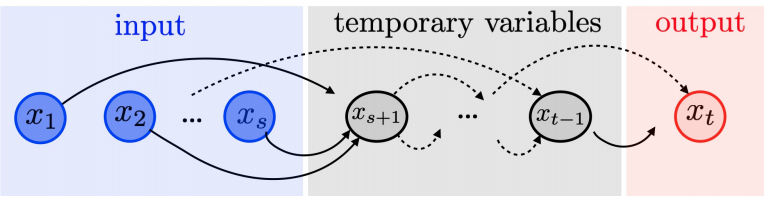
\includegraphics[width=.8\textwidth]{computational_graph.png}\\
 \vspace{0.3cm}
 \begin{footnotesize}
  SOURCE:~\citeonline[p.~31]{peyre}.
 \end{footnotesize}
 \label{fig:compgraph}
\end{figure}

Assuming that \(f\) is implemented in an algorithm, the goal is to
compute the derivatives
\begin{align*}
 &\frac{\partial f(\bm{x})}{\partial\bm{x}_{k}}\in
  \mathbb{R}^{n_{t} \times n_{k}},\\
 &\text{for a numerical algorithm (succession of functions)
        of the form}\\
 &\forall~k = s + 1,~\dots,~t,\quad
  \bm{x}_{k} = f_{k}(\bm{x}_{1},~\dots,~\bm{x}_{k-1}),
\end{align*}
where \(f_{k}\) is a function which only depends on the previous
variables. The computational graph as in \autoref{fig:compgraph}, has
the role of represent the linking of the variables involved in \(f_{k}\)
to \(\bm{x}_{k}\). The evaluation of \(f(\bm{x})\) corresponds to a
forward traversal of this graph.

Now, how we evaluate \(f\) through the graph? Via one of the AD modes.

\subsection{Forward Mode}

The forward mode correspond to the usual way of computing differentials.
The method initialize with the derivative of the input nodes
\[
 \frac{\partial\bm{x}_{1}}{\partial\bm{x}_{1}} =
 \text{Id}_{n_{1} \times n_{1}},\quad
 \frac{\partial\bm{x}_{2}}{\partial\bm{x}_{1}} =
 \bm{0}_{n_{2} \times n_{1}},\quad
 \frac{\partial\bm{x}_{s}}{\partial\bm{x}_{1}} =
 \bm{0}_{n_{s} \times n_{1}},
\]
and then iteratively make use of the following recursion formula
\begin{align*}
 &\forall~k = s + 1,~\dots,~t,\\
 &\frac{\partial\bm{x}_{k}}{\partial\bm{x}_{1}} =
  \sum_{l~\in~\text{father}(k)}
  \frac{\partial\bm{x}_{k}}{\partial\bm{x}_{l}}\times
  \frac{\partial\bm{x}_{l}}{\partial\bm{x}_{1}} =
  \sum_{l~\in~\text{father}(k)}
  \frac{\partial}{\partial\bm{x}_{l}}
  f_{k}(\bm{x}_{1},~\dots,~\bm{x}_{k-1})\times
  \frac{\partial\bm{x}_{l}}{\partial\bm{x}_{1}}.
\end{align*}
The notation ``father(\(k\))'' denotes the nodes \(l < k\) of the graph
that are connected to \(k\). We make use of \citeonline[p.~32]{peyre}'s
simple example.

\noindent\textbf{Example.}\hspace{.5cm}
Consider the function
\[
 f(x, y) = y\log(x) + \sqrt{y\log(x)}
\]
with the corresponding computational graph being displayed in
\autoref{fig:excompgraph}.

\begin{figure}[H]
 \setlength{\abovecaptionskip}{.0001pt}
 \caption{EXAMPLE OF A SIMPLE COMPUTATIONAL GRAPH}
 \vspace{0.3cm}\centering
 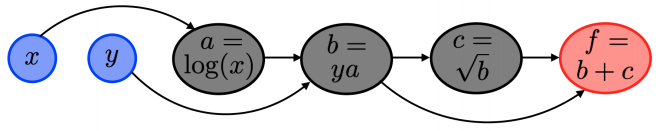
\includegraphics[width=.8\textwidth]{ex-computational_graph.png}\\
 \vspace{0.3cm}
 \begin{footnotesize}
  SOURCE:~\citeonline[p.~33]{peyre}.
 \end{footnotesize}
 \label{fig:excompgraph}
\end{figure}

The forward mode iterations to compute the derivative w.r.t. \(x\)
following the computational graph, are given by
\begin{align*}
 \frac{\partial x}{\partial x} &= 1, \quad
 \frac{\partial y}{\partial x} = 0\\
 \frac{\partial a}{\partial x} &=
 \frac{\partial a}{\partial x} \frac{\partial x}{\partial x} =
 \frac{1}{x} \frac{\partial x}{\partial x} \qquad
 &\{x \mapsto a = \log(x)\}\\
 \frac{\partial b}{\partial x} &=
 \frac{\partial b}{\partial a} \frac{\partial a}{\partial x} +
 \frac{\partial b}{\partial y} \frac{\partial y}{\partial x} =
 y \frac{\partial a}{\partial x} + 0 \qquad
 &\{(y, a) \mapsto b = ya\}\\
 \frac{\partial c}{\partial x} &=
 \frac{\partial c}{\partial b} \frac{\partial b}{\partial x} =
 \frac{1}{2\sqrt{b}} \frac{\partial b}{\partial x} \qquad
 &\{b \mapsto c = \sqrt{b}\}\\
 \frac{\partial f}{\partial x} &=
 \frac{\partial f}{\partial b} \frac{\partial b}{\partial x} +
 \frac{\partial f}{\partial c} \frac{\partial c}{\partial x} =
 1 \frac{\partial b}{\partial x} + 1 \frac{\partial c}{\partial x}
 \qquad &\{(b, c) \mapsto f = b + c\}
\end{align*}
To compute the derivative w.r.t. \(y\) we run another forward process
\begin{align*}
 \frac{\partial x}{\partial y} &= 0, \quad
 \frac{\partial y}{\partial y} = 1\\
 \frac{\partial a}{\partial y} &=
 \frac{\partial a}{\partial x} \frac{\partial x}{\partial y} = 0 \qquad
 &\{x \mapsto a = \log(x)\}\\
 \frac{\partial b}{\partial y} &=
 \frac{\partial b}{\partial a} \frac{\partial a}{\partial y} +
 \frac{\partial b}{\partial y} \frac{\partial y}{\partial y} =
 0 + a \frac{\partial y}{\partial y}\qquad
 &\{(y, a) \mapsto b = ya\}\\
 \frac{\partial c}{\partial y} &=
 \frac{\partial c}{\partial b} \frac{\partial b}{\partial y} =
 \frac{1}{2\sqrt{b}} \frac{\partial b}{\partial y} \qquad
 &\{b \mapsto c = \sqrt{b}\}\\
 \frac{\partial f}{\partial y} &=
 \frac{\partial f}{\partial b} \frac{\partial b}{\partial y} +
 \frac{\partial f}{\partial c} \frac{\partial c}{\partial y} =
 1 \frac{\partial b}{\partial y} + 1 \frac{\partial c}{\partial y}
 \qquad &\{(b, c) \mapsto f = b + c\}
\end{align*}

\subsection{Reverse Mode}

Instead of evaluating the differentials for all the input nodes, which
is problematic for a large number of nodes, the reverse mode evaluates
the differentials of the output node w.r.t. all the inner nodes.

The method is based on a backward adjoint chain rule and initialize with
the derivative of the final node
\[
 \frac{\partial\bm{x}_{t}}{\partial\bm{x}_{t}} =
 \text{Id}_{n_{t} \times n_{t}},
\]
and then from the last to the first node, iteratively make use of the
following recursion formula
\begin{align*}
 &\forall~k = t - 1,~t - 2,~\dots,~1,\\
 &\frac{\partial\bm{x}_{t}}{\partial\bm{x}_{k}} =
  \sum_{m~\in~\text{son}(k)}
  \frac{\partial\bm{x}_{t}}{\partial\bm{x}_{m}}\times
  \frac{\partial\bm{x}_{m}}{\partial\bm{x}_{k}} =
  \sum_{m~\in~\text{son}(k)}
  \frac{\partial\bm{x}_{t}}{\partial\bm{x}_{m}}\times
  \frac{\partial}{\partial\bm{x}_{k}}
  f_{m}(\bm{x}_{1},~\dots,~\bm{x}_{m}).
\end{align*}
The notation ``son(\(k\))'' denotes the nodes \(m < k\) of the graph
that are connected to \(k\). To be clear, the same simple example.

\noindent\textbf{Example.}\hspace{.5cm}
Consider again the function
\[
  f(x, y) = y\log(x) + \sqrt{y\log(x)}.
\]
The iterations of the reverse mode are given by
\begin{align*}
 \frac{\partial f}{\partial f} &= 1\\
 \frac{\partial f}{\partial c} &=
 \frac{\partial f}{\partial f} \frac{\partial f}{\partial c} =
 \frac{\partial f}{\partial f} 1\qquad &\{c \mapsto f = b + c\}\\
 \frac{\partial f}{\partial b} &=
 \frac{\partial f}{\partial c} \frac{\partial c}{\partial b} +
 \frac{\partial f}{\partial f} \frac{\partial f}{\partial b} =
 \frac{\partial f}{\partial c} \frac{1}{2\sqrt{b}} +
 \frac{\partial f}{\partial f} 1\qquad
 &\{b \mapsto c = \sqrt{b},~b \mapsto f = b + c\}\\
 \frac{\partial f}{\partial a} &=
 \frac{\partial f}{\partial b} \frac{\partial b}{\partial a} =
 \frac{\partial f}{\partial b} y\qquad &\{a \mapsto b = ya\}\\
 \frac{\partial f}{\partial y} &=
 \frac{\partial f}{\partial b} \frac{\partial b}{\partial y} =
 \frac{\partial f}{\partial b} a \qquad &\{y \mapsto b = ya\}\\
 \frac{\partial f}{\partial x} &=
 \frac{\partial f}{\partial a} \frac{\partial a}{\partial x} =
 \frac{\partial f}{\partial a} \frac{1}{x} \hspace{6.5cm}
 &\{x \mapsto a = \log(x)\}
\end{align*}
This is the advantage of reverse mode over the forward mode. A single
traversal over the computational graph allows to compute both
derivatives w.r.t. \(x\) and \(y\), while the forward mode necessities
two processes.

An drawback of the reverse mode is the need to store the entire
computational graph, which is needed for the reverse sweep. In
principle, storage of this graph is not too difficult to implement.
However, the main benefit of AD is higher accuracy, and in many
applications the cost is not critical.

\section{TMB: TEMPLATE MODEL BUILDER}
\label{cap:tmb}

Note that the goal of AD is not to define an efficient computational
graph, it is up to the user to provide it. However, computing an
efficient graph associated to a mathematical formula is a complicated
combinatorial problem. Thus, since our goal is to be able to fit our
desired statistical models, a computational tool able to efficiently
define and implement this computational graph is make necessary. To
solve this and many other tasks we have the Template Model Builder
(TMB), developed by \citeonline{TMB}.

TMB \url{ http://tmb-project.org} is an \texttt{R} \cite{R21} package
for fitting statistical latent variable models to data, inpired by AD
Model Builder (ADMB) \cite{ADMB}. ADMB is a statistical application for
fitting nonlinear statistical models and solve optimization problems,
that implements AD using \texttt{C++} classes and a native template
language. Unlike most \texttt{R} packages, in TMB the model is
formulated in \texttt{C++}. This characteristic provides great
flexibility but requires some familiarity with the
\texttt{C}/\texttt{C++} programming language.

With TMB a user should be able to quickly implement complex latent
effect models through simple \texttt{C++} templates. As an illustrative
example let us consider an simple mixed logistic regression i.e., a
binomial GLMM with a logistic link function. The latent structure is in
the context of repeated measures, the same subject is observed three
times. Trying to keep it simple, no covariates. A hierarchical model's
description is given by
\begin{align*}
 y_{ij} \mid u_{i} &\sim \text{Binomial}(n, p_{ij})\\
            u_{i} &\sim \text{Normal}(0, 1)\\
 g(p_{ij}) = \text{logit}(p_{ij}) &=
 \log\frac{p_{ij}}{1 - p_{ij}} = \beta + u_{i}\\
 p_{ij} &= \frac{\exp\{\beta + u_{i}\}}{1 + \exp\{\beta + u_{i}\}},\quad
 i~\text{the subject},~j~\text{the subject observation}~(1,2,3).
\end{align*}
The TMB implementation of this model is provided in Figure
\autoref{fig:tmbex-p1}.

To keep the coherence would be more adequate to fit here a multinomial
model. However, I want to show you that in TMB we can also simulate data
from the model but not all \texttt{r}-distributions are implemented, as
is the case of the multinomial. For this reason, a binomial model was
the choice. An even easier implementation of a logistic model is
available in TMB, called \texttt{dbinom\_robust()}, where we pass
directly the \(\text{logit}(\cdot)\) but we do not have an
\texttt{rbinom\_robust()} implementation available. Just for the sake of
completeness, in Figure \autoref{fig:tmbex-p2} we have the \texttt{R}
code showing how to manipulate the \texttt{C++} model template in terms
of object definitions and parameters estimation and extraction for the
logistic mixed model.

In this chapter we describe step-by-step all the processes involved in
the formulation and parameter estimation of a GLMM. With TMB all this is
put in practice in an efficient and robust fashion. The user needs to
provide the negative joint log-likelihood function writing in a
\texttt{C++} template as exemplified in Figure \autoref{fig:tmbex-p1},
using specialized macros that pass the parameters, latent effects and
data from \texttt{R}, as exemplified in Figure \autoref{fig:tmbex-p2}.

When the model presents latent effects, during the model template
compilation the latent effects are integrated out via an efficient
Laplace approximation routine with the inner optimization made by a
Newton algorithm, and the negative marginal log-likelihood gradient is
computed, via AD. The negative marginal log-likelihood is returned into
an \texttt{R} object that can then be optimized using the user's
favorite quasi-Newton routine, available in \texttt{R}. All these
procedures are briefly exemplified for a logistic mixed model in Figure
\autoref{fig:tmbex-p1} and Figure \autoref{fig:tmbex-p2}.

To accomplish all that, TMB combines some state-of-art software
\begin{itemize}
 \item \texttt{CppAD}, a \texttt{C++} AD
       package \url{https://coin-or.github.io/CppAD/};

 \item \texttt{Eigen} \cite{eigen}, a \texttt{C++} templated
       matrix-vector library;

 \item \texttt{CHOLMOD}, \texttt{C} sparse matrix routines available
       from \texttt{R}, used to obtain an efficient implementation of
       the Laplace approximation with exact
       derivatives \url{https://developer.nvidia.com/cholmod};

 \item Parallelism
       through \texttt{BLAS} \url{http://www.netlib.org/blas/},
       a \texttt{Fortran} tuned set of Basic Linear Algebra Subprograms;
\end{itemize}

\begin{figure}[H]
 \setlength{\abovecaptionskip}{.0001pt}
 \caption{\texttt{R} CODE FOR THE TMB IMPLEMENTATION OF A LOGISTIC MIXED
          MODEL}
 \vspace{0.3cm}\centering
 \lstinputlisting[lastline=44]{modules/exampleTMB.R}
 \begin{footnotesize}
  SOURCE: The author~(2021).
 \end{footnotesize}
 \label{fig:tmbex-p1}
\end{figure}

\begin{itemize}
 \item \texttt{Matrix} \cite{Matrix}, a rich hierarchy sparse and dense
       matrix classes and methods
       using \texttt{LAPACK} \url{http://www.netlib.org/lapack/}
       and \texttt{SuiteSparse} \url{https://sparse.tamu.edu/}
       libraries.
\end{itemize}

\begin{figure}[H]
 \setlength{\abovecaptionskip}{.0001pt}
 \caption{\texttt{R} CODE FOR THE MODEL FITTING OF A LOGISTIC MIXED
          MODEL WRITTEN IN TMB}
 \vspace{0.3cm}\centering
 \lstinputlisting[firstline=46]{modules/exampleTMB.R}
 \begin{footnotesize}
  SOURCE: The author~(2021).
 \end{footnotesize}
 \label{fig:tmbex-p2}
\end{figure}
\noindent
An overview of the pachage design is shown in
\autoref{fig:tmbpackdesign}.

\begin{figure}[H]
 \setlength{\abovecaptionskip}{.0001pt}
 \caption{TMB PACKAGE DESIGN}
 \vspace{0.35cm}\centering
 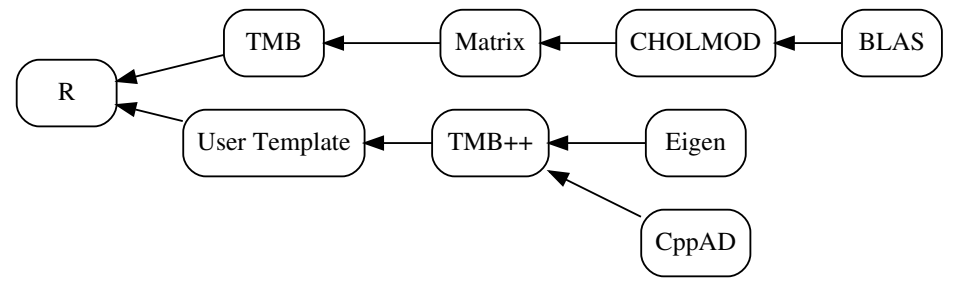
\includegraphics[width=0.85\textwidth]{tmb_package_design.png}\\
 \vspace{0.1cm}
 \begin{footnotesize}
  SOURCE:~\citeonline{TMB}.
 \end{footnotesize}
 \label{fig:tmbpackdesign}
\end{figure}
\noindent
Reinforcing, some key characteristics are
\begin{itemize}
 \item TMB employs AD to calculate first and second order derivatives of
       the log-likelihood function or of any objective function written
       in \texttt{C++};

 \item The objective function, and its derivatives, can be called
       from \texttt{R}. Hence, parameter estimation
       via \texttt{base::optim()} or \texttt{base::nlminb()} is easy to
       be performed;

 \item Standard deviations of any parameter, or derived parameter, can
       be obtained via the \textit{delta method} \cite{deltamethod}
       implemented in \texttt{TMB::sdreport()}.
\end{itemize}

Here we focus on GLMMs, but basically any statistical model with a
latent structure (or not), linear (or not), can be fitted with TMB. In
times of \textit{big data} and with the TMB's authors having a
professional preference for state-space and spatial models, TMB has also
automatic sparseness detection and some other nice built tools. Pre and
post-processing of data should be done in \texttt{R}.

A TMB Users' mailing list exists, and it is extremely helpful for taking
doubts and questions \url{https://groups.google.com/g/tmb-users}. Also,
a very didactic and comprehensive documentation with several examples is
available online
\url{https://kaskr.github.io/adcomp/_book/Tutorial.html}.

% END ==================================================================
